% !TeX root = ../main.tex

\chapter{Experimental Setup}\label{chapter:experimental-setup}

The experimental setup was designed to validate the control concept on a physical platform with accurate ground-truth feedback and synchronized onboard telemetry.
The objectives were (i) to verify that the INDI controller maintains stable flight under aerodynamic loading and (ii) to record sufficient data for quantitative assessment of tracking accuracy and thrust behavior.

\section{Hardware Configuration}\label{sec:hardware}

The test vehicle is the X-wing quadrotor described in Chapter~\ref{chapter:platform-design} with a total mass of \SI{2.5}{\kilogram}.
Each T-MOTOR VELOX V2808 motor equipped with HQProp 7×3.5×3 propellers produces up to \SI{22}{\newton} static thrust, giving a thrust-to-weight ratio of 3.6.
The motor layout and rotation directions follow the conventional ``X'' configuration (Figure~\ref{fig:motor_configuration}).

The aerodynamic surfaces follow a NACA 0015 profile with \SI{0.45}{\meter} span and \SI{0.25}{\meter} chord at $\pm\SI{45}{\degree}$ dihedral/anhedral.
The total projected wing area is \SI{0.318}{\meter\squared}.
The center of gravity coincides with the geometric center, minimizing trim moments.

Two identical 6\,S \SI{1400}{\milli\ampere\hour} Li-Po batteries are connected in parallel, yielding \SI{2.8}{\ampere\hour} effective capacity.
The avionics stack consists of a Kakute H7 v1.5 flight controller and a Jetson Orin Nano (8\,GB) companion computer communicating via UART over MAVLink.
The flight controller runs modified Betaflight firmware capable of reporting motor RPM and battery voltage through MAVLink for logging.

\begin{figure}[htbp]
\centering
\begin{tikzpicture}[scale=1.5]
    % Define motor positions (X configuration)
    \coordinate (M1) at (1.5, -1.5);  % Bottom right
    \coordinate (M2) at (1.5, 1.5);   % Top right
    \coordinate (M3) at (-1.5, -1.5); % Bottom left
    \coordinate (M4) at (-1.5, 1.5);  % Top left
    
    % Draw center cross (arms)
    \draw[very thick, gray!50] (-1.5, -1.5) -- (1.5, 1.5);
    \draw[very thick, gray!50] (-1.5, 1.5) -- (1.5, -1.5);
    
    % Draw motors as circles with rotation arrows
    % Motor 1 (Bottom Right) - CW
    \draw[thick, fill=gray!20] (M1) circle (0.5cm);
    \node[font=\Large\bfseries] at (M1) {1};
    \draw[->, thick, TUMBlue, line width=1.5pt] (M1) ++(315:0.4cm) arc (315:225:0.4cm);
    
    % Motor 2 (Top Right) - CCW
    \draw[thick, fill=gray!20] (M2) circle (0.5cm);
    \node[font=\Large\bfseries] at (M2) {2};
    \draw[->, thick, TUMBlue, line width=1.5pt] (M2) ++(45:0.4cm) arc (45:135:0.4cm);
    
    % Motor 3 (Bottom Left) - CCW
    \draw[thick, fill=gray!20] (M3) circle (0.5cm);
    \node[font=\Large\bfseries] at (M3) {3};
    \draw[->, thick, TUMBlue, line width=1.5pt] (M3) ++(225:0.4cm) arc (225:315:0.4cm);
    
    % Motor 4 (Top Left) - CW
    \draw[thick, fill=gray!20] (M4) circle (0.5cm);
    \node[font=\Large\bfseries] at (M4) {4};
    \draw[->, thick, TUMBlue, line width=1.5pt] (M4) ++(135:0.4cm) arc (135:45:0.4cm);
    
    % Forward direction arrow
    \draw[->, very thick, red, line width=2pt] (0, 2.5) -- (0, 3.2);
    \node[red, font=\Large\bfseries] at (0, 3.6) {Forward};
\end{tikzpicture}
\caption{Motor configuration and numbering convention. Blue arrows indicate rotation direction.}
\label{fig:motor_configuration}
\end{figure}

\begin{figure}[htbp]
\centering
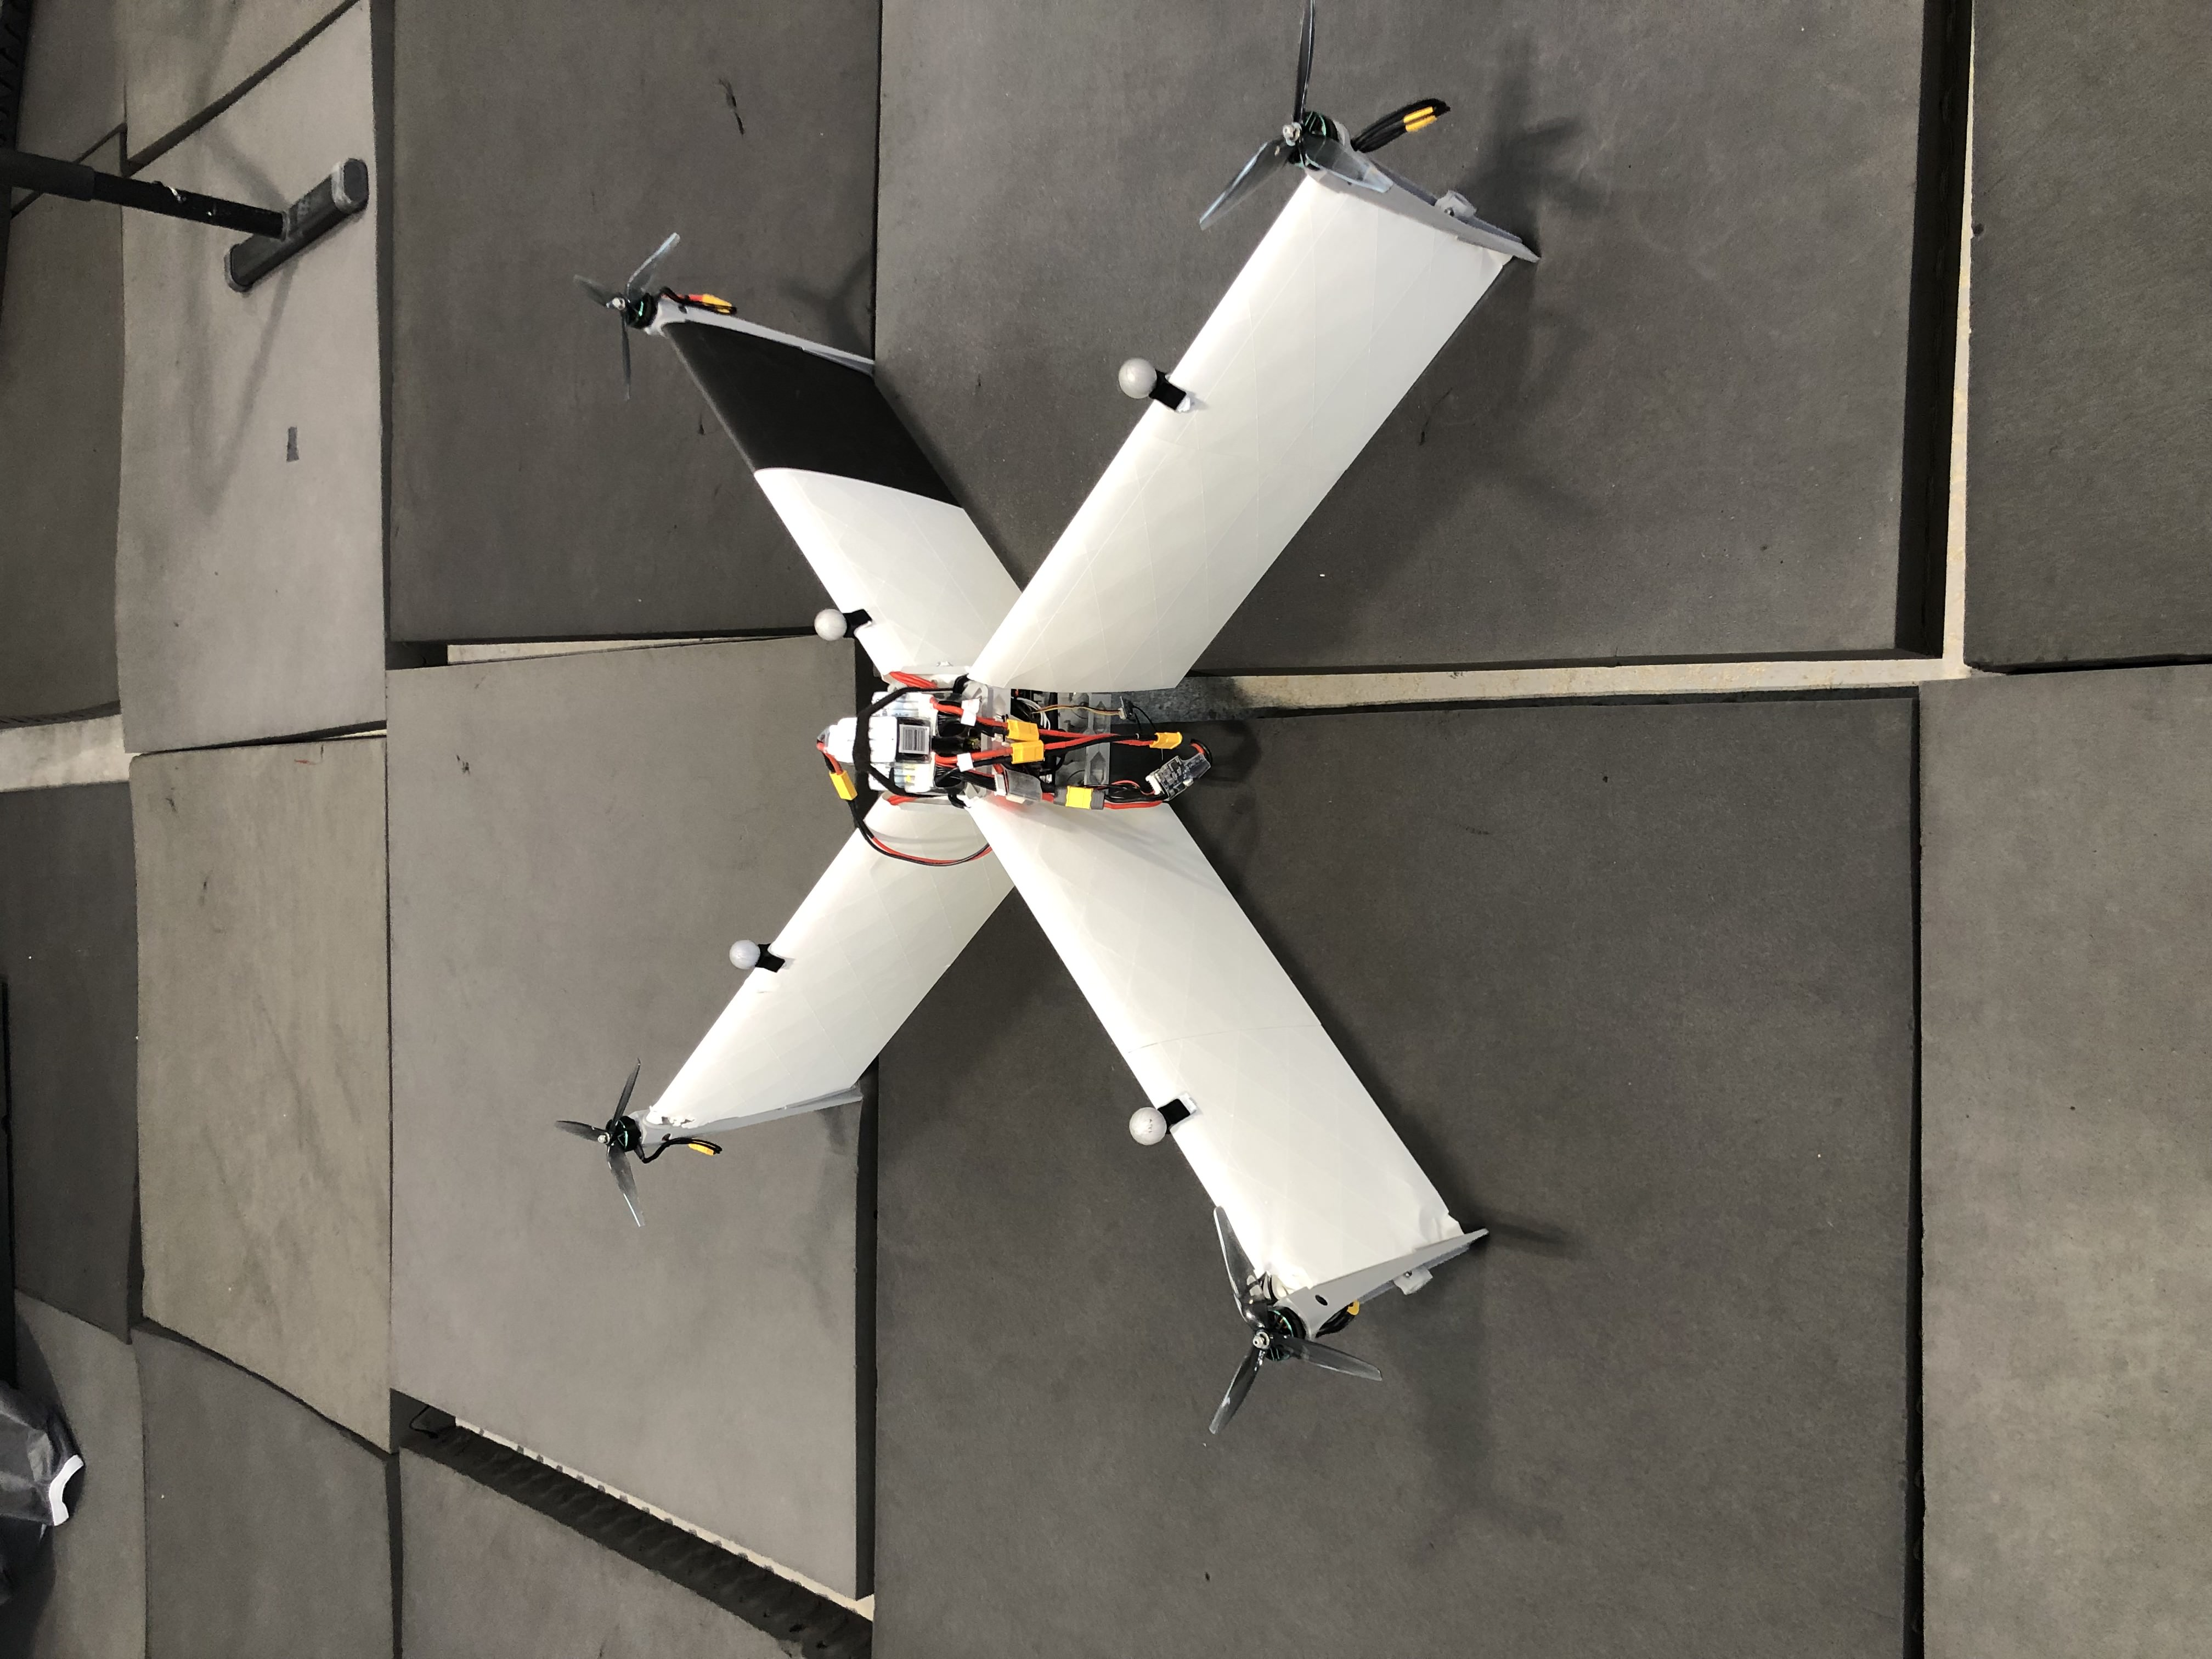
\includegraphics[width=0.7\textwidth,angle=-90]{figures/drone_hover.jpg}
\caption{The experimental X-wing quadrotor platform in the Vicon arena.}
\label{fig:xwing_platform}
\end{figure}

\section{Platform Variants}\label{sec:platform-variants}

Two airframe variants were used:
\begin{itemize}
\item \textbf{Baseline}: The original $\pm\SI{45}{\degree}$ NACA 0015 X-wing design developed in this thesis.
\item \textbf{Improved}: An AG25 cambered-airfoil version with $\pm\SI{20}{\degree}$ dihedral developed by Pablo Kirby (2025).\footnote{Pablo Kirby, \textit{Bachelor Thesis}, TUM, 2025.}
\end{itemize}

Both share identical propulsion, electronics, and control code, enabling fair aerodynamic comparison.
All controller tuning and test results presented in this thesis refer to the baseline variant unless explicitly stated.

\section{Thrust Characterization}\label{sec:thrust-characterization}

Static thrust measurements were performed on a custom rig using a six-axis Rokubi Mini force--torque sensor (Figure~\ref{fig:force_test_stand}).
A single motor was driven through the same Betaflight/DShot interface used in flight to ensure identical timing behavior.

A total of 975 samples were recorded across the full throttle range under the 6\,S 2\,P configuration to include battery voltage sag.
The resulting quadratic mapping
\begin{equation}
T = 5.15\times 10^{-2}\,\text{RPM}^2 - 0.09\,\text{RPM}
\end{equation}
achieved $R^2=0.997$.
This mapping was integrated into the controller for thrust estimation and energy-related post-analysis.

\begin{figure}[h]
\centering
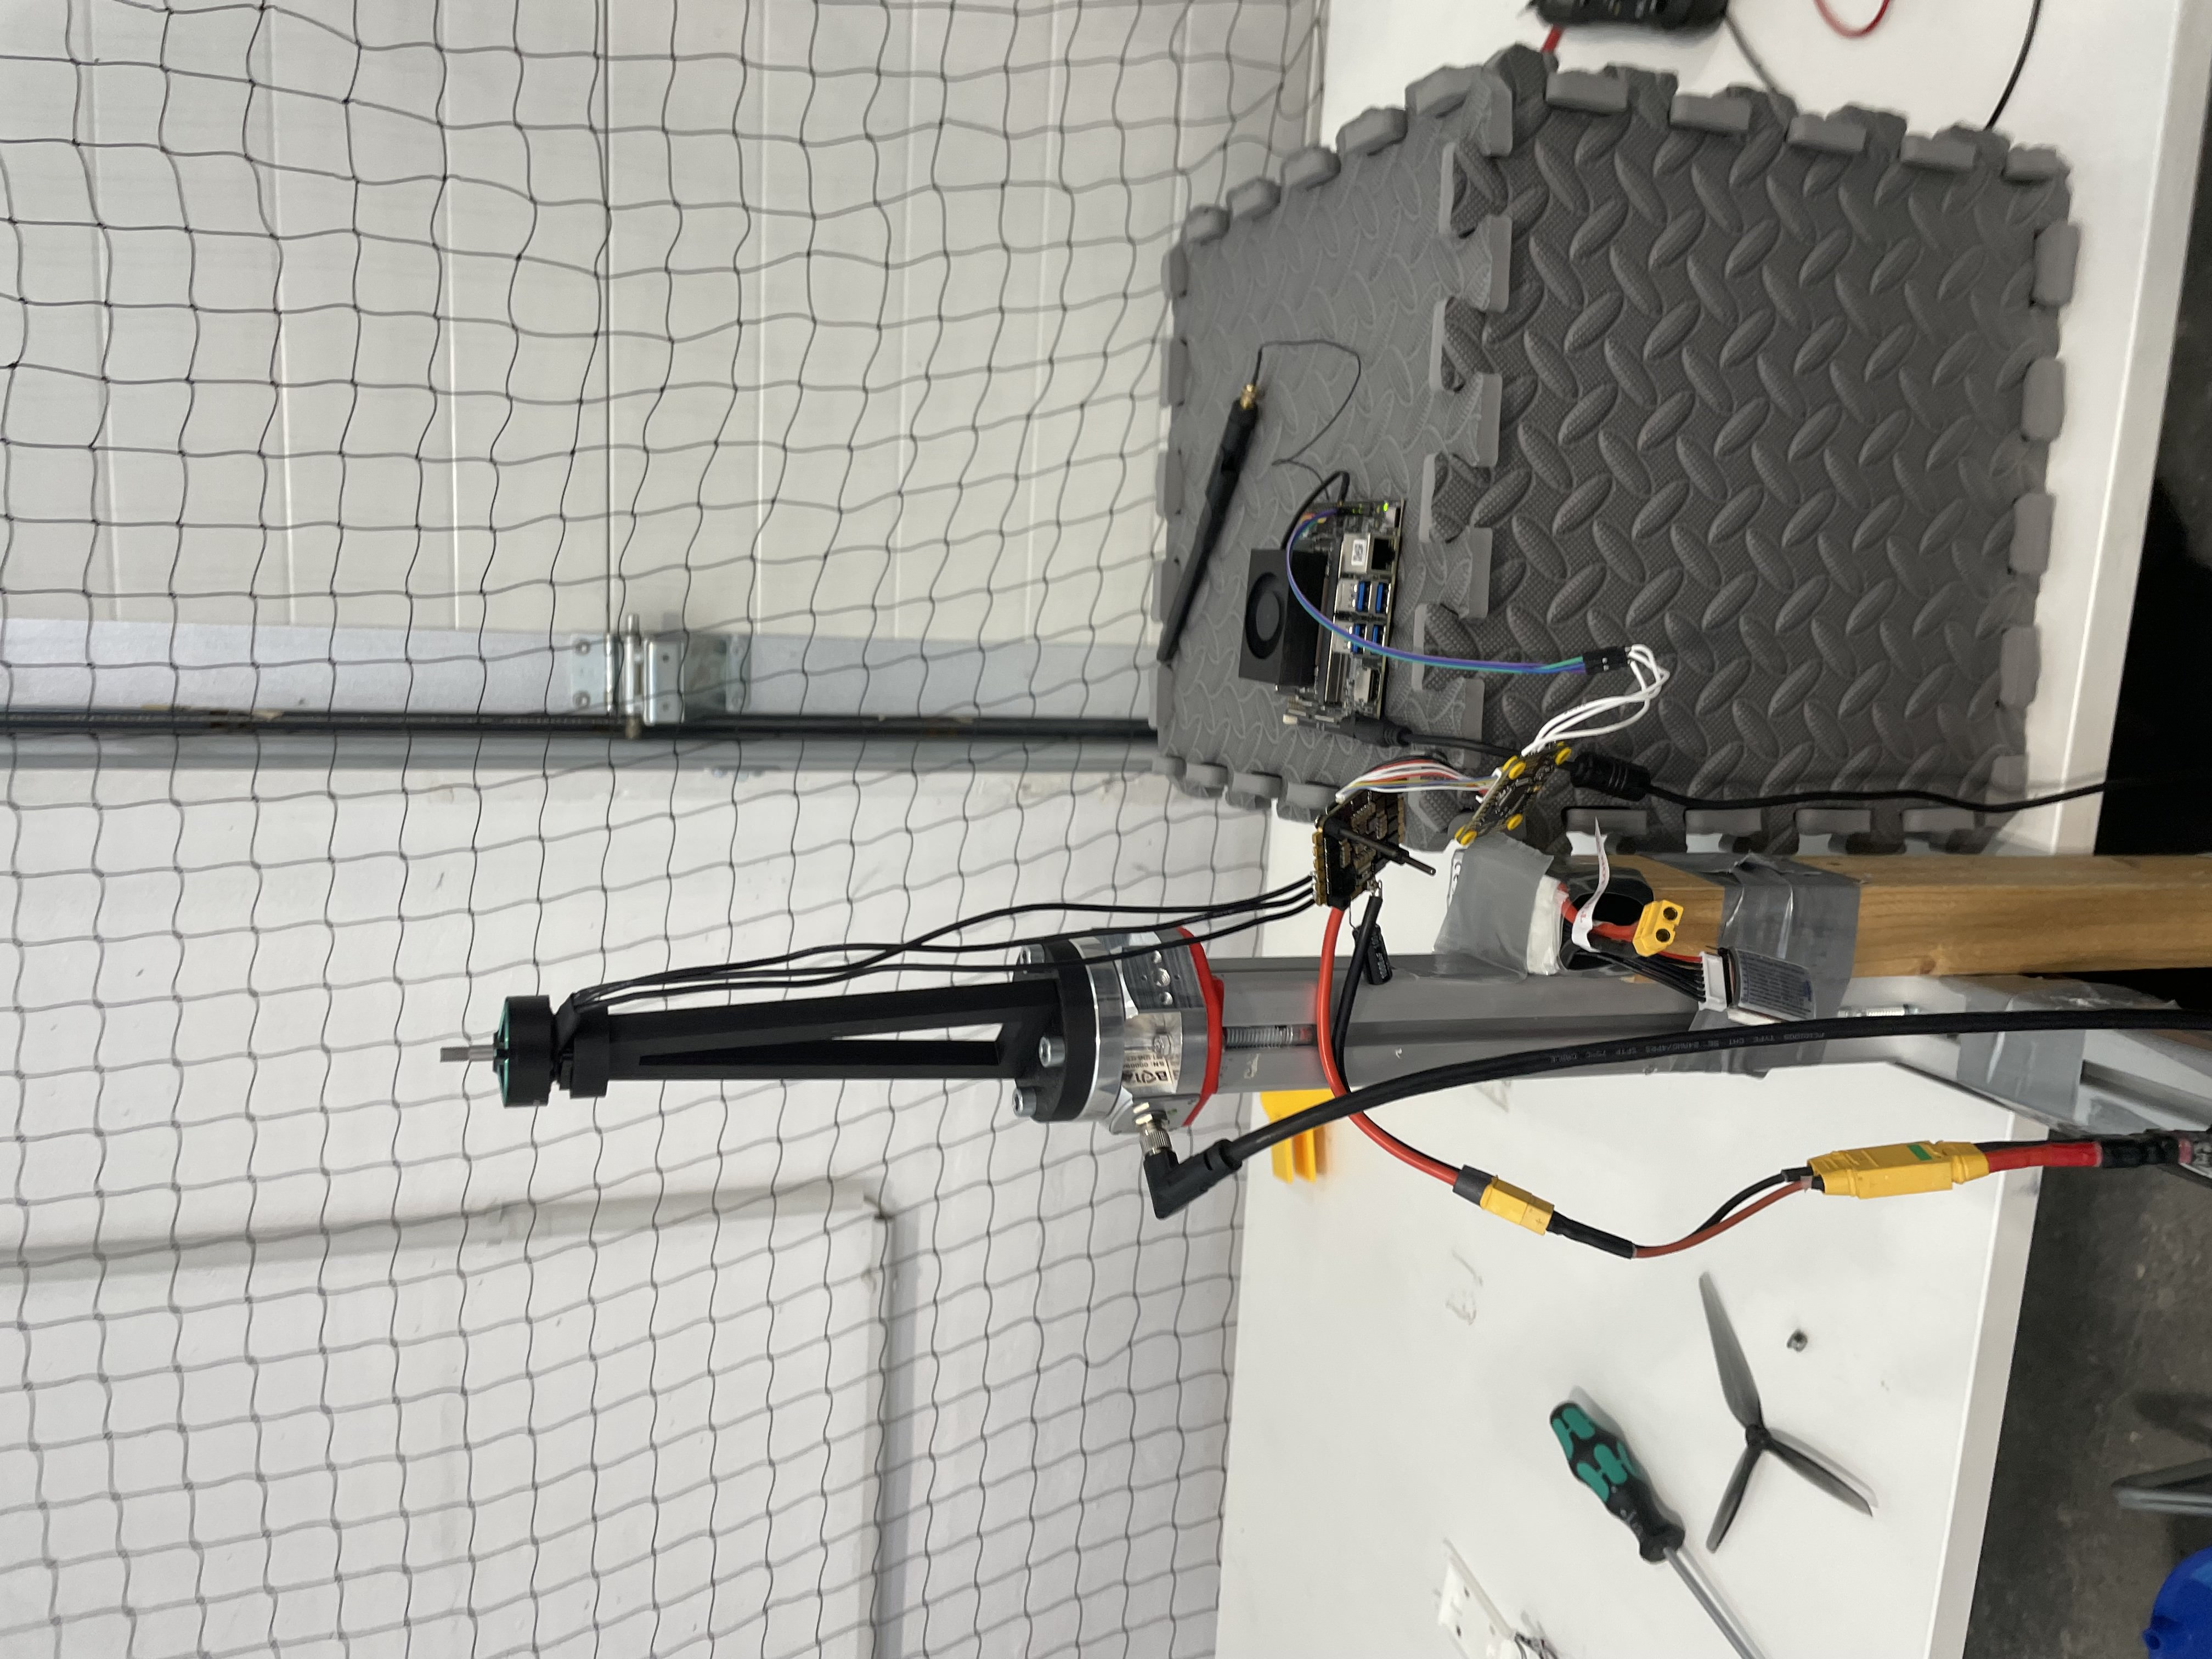
\includegraphics[width=0.7\linewidth,angle=-90]{figures/force_test_stand.jpg}
\caption{Static thrust characterization test stand with motor mounted on Rokubi Mini force--torque sensor.}
\label{fig:force_test_stand}
\end{figure}

\section{Avionics and Communication}\label{sec:avionics}

All control logic ran on the Jetson companion computer under ROS~1 (Noetic).
The geometric + INDI stack executed at 300\,Hz inner-loop and 300\,Hz outer-loop frequencies.
Data streams between Jetson and Kakute used MAVLink~2 over UART (921\,kbit/s).

The flight controller relayed IMU data (8\,kHz) and per-motor RPM to the Jetson.
End-to-end command latency, measured via timestamp correlation, was $\approx 12$\,ms—short enough to satisfy the INDI assumption that disturbance changes are slow relative to the control rate.

\section{Measurement and Logging}\label{sec:measurement}

Ground-truth position and attitude were provided by Vicon motion-capture systems operating at 200\,Hz.
For agility trials, the $7 \times 8$\,m Munich arena was used; for efficiency and high-speed tests, the $60 \times 45$\,m AIDA Hall at Reutlingen University (Figure~\ref{fig:aida_hall}).
Both datasets were timestamp-synchronized with onboard telemetry via NTP and merged in rosbag format.

Logged variables included:
\begin{itemize}
\item Position, velocity, attitude (Vicon)
\item Angular rates and linear accelerations (IMU)
\item Motor RPM and control commands
\item Battery voltage
\end{itemize}

These channels provided all necessary signals for thrust estimation, trajectory-tracking evaluation, and disturbance-rejection analysis.

\begin{figure}[h]
\centering
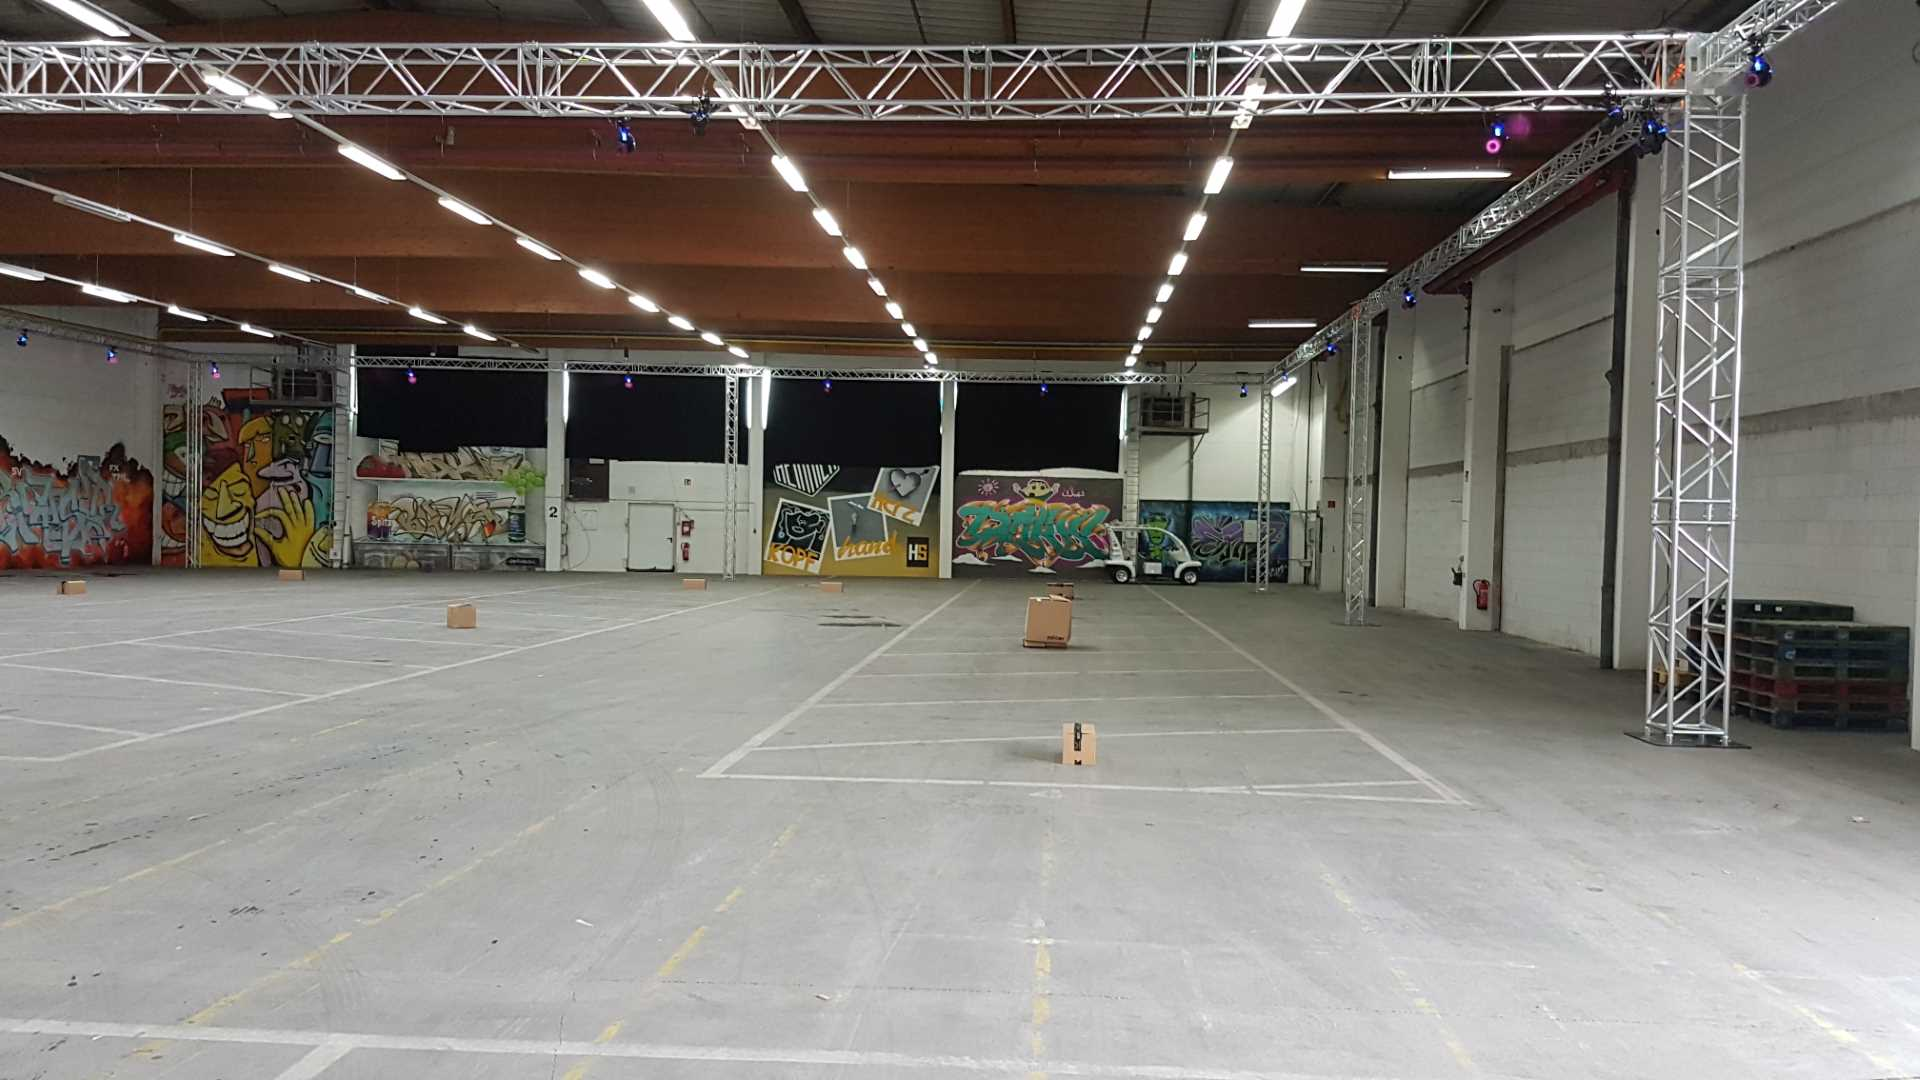
\includegraphics[width=0.85\linewidth]{figures/aida_hall.jpg}
\caption{AIDA Hall test facility used for efficiency trials (image credit: Reutlingen University~\cite{AIDAHallPhoto2024}).}
\label{fig:aida_hall}
\end{figure}

\section{Experimental Protocol}\label{sec:protocol}

Each flight consisted of an autonomous take-off, hover stabilization, and a pre-programmed trajectory (step or circular).
Manual override from the ground station was available for safety.
All maneuvers were repeated until consistent trajectories and no external airflow disturbances were observed.
Each dataset was verified for timing consistency and outliers before analysis.

\section{Data Quality and Uncertainty}\label{sec:data-quality}

Sensor noise levels were assessed via static logs: IMU acceleration noise $\approx 0.03$\,m\,s$^{-2}$ rms; Vicon position uncertainty $\pm 2$\,mm; timestamp jitter $< 5$\,ms.
No measurable bias drift affected the evaluation interval ($\leq 5$\,min per flight).
These figures ensure that the reported tracking errors in Chapter~\ref{chapter:experiments-evaluation} exceed measurement noise by at least one order of magnitude.

\section{Summary}\label{sec:exp-setup-summary}

The experimental setup provides synchronized, high-fidelity data for validating the control approach.
It achieves sufficient accuracy to resolve sub-decimeter trajectory errors and verify that the INDI controller can stabilize and track trajectories under unmodeled aerodynamic disturbances.

% --- References used in this chapter ---
% \cite{AIDAHallPhoto2024}

